%
% ---------- header -----------------------------------------------------------
%
% project       kaneton
%
% license       kaneton
%
% file          /home/mycure/kaneton/view/book/kaneton/terminology.tex
%
% created       julien quintard   [mon jun 18 15:45:43 2007]
% updated       julien quintard   [sun dec 16 17:24:00 2007]
%

%
% ---------- terminology ------------------------------------------------------
%

\chapter{Terminology}
\label{chapter:terminology}

In this chapter the kaneton terminology is detailed. This terminology is
quite different from other kernel and operating system projects in many ways.

\newpage

%
% ---------- text -------------------------------------------------------------
%

The kaneton terminology was introduced for making communication easier.
Indeed, it is sometimes difficult to communicate about a technical
field like kernels design and development with terms as specific as
``architecture-independent soure code'', ``module of the \textit{mod}
service'', ``contiguous area of free virtual memory'' etc.

The reader should notice that these terms are complex and a bit confusing
when used together in the same sentence. Therefore, kaneton people decided to
introduce a well defined terminology to make things clear and more
understandable.

This section tries to detail the terminology inherent to the kaneton project
by classifying the terms according to their context. The remaining of
this chapter is divided into two categories: \textit{Design} and
\textit{Implementation}. The \textit{Design} section contains the kaneton
general terminology while the \textit{Implementation} section contains some
naming rules the kaneton microkernel research project implementation follows.

%
% design
%

\section{Design}

Although microkernel-based operating systems are, by nature, modular, kaneton
people wanted the microkernel itself to be modular, subdivided into logical
parts. This subdivision was introduced to make the whole microkernel clearer
and more understandable.

The kaneton microkernel is thus divided into \textbf{managers}. These
managers are generally responsible for a \textbf{kaneton object} type but there
exist managers which manage something else or just create an abstraction over
other kaneton managers. A kaneton object represents a logical and fundamental
kernel entity. These objects are described later in this section.

\textit{Figure \ref{figure:managers-organisation}} illustrates the
decomposition of the microkernel into multiples managers.

\begin{figure}[h]
  \begin{center}
    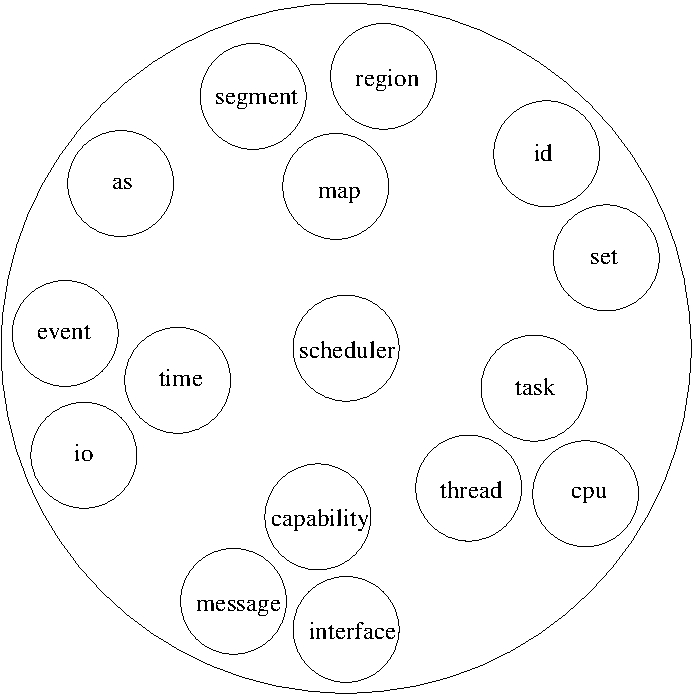
\includegraphics[scale=0.7]{\path/figures/managers-organisation.pdf}
    \caption{kaneton managers.}
    \label{figure:managers-organisation}
  \end{center}
\end{figure}

Note that this decomposition has no direct relation with the \textit{Object
Programming} paradigm. Indeed, even if kaneton designers tried to reduce the
dependencies between the managers, some managers remain intrusive as they
access the data structures of one or more other managers.

A kaneton object represents a kernel entity. Every object is identified by
a \textbf{kaneton identifier} and protected by a \textbf{kaneton capability}
over the operating and distributed system.

Below are listed the most important objects:

\begin{itemize}
  \item
    A \textbf{segment} represents a continuous area of physical memory.
  \item
    A \textbf{region} represents a continuous area of virtual memory which
    maps a part of or a whole \textit{segment}.
  \item
    An \textbf{as} or \textbf{address space} represents a set of physical
    memory areas which can potentially be accessed through a set of virtual
    memory addresses.

    \-

    An \textit{as} is composed of a set of \textit{segments} and a set of
    \textit{regions}.
  \item
    A \textbf{task} represents a complete execution context.

    \-

    However, a \textit{task} is not an active entity as it is not the
    one scheduled. Indeed, a \textit{task} is actually composed of an
    \textit{address space} and one or more \textit{threads}.
  \item
    A \textbf{thread} represents the active execution context in a
    \textit{task}.
  \item
    An \textbf{event} describes an external event including hardware
    events like interrupts as well as software events also known as
    \textit{system calls} or \textit{syscalls}.
  \item
    \textbf{Message}s are used for communicating betweens tasks.
\end{itemize}

The reader should notice that there is a hierarchical relation between
these objects as it is illustrated by \textit{Figure
\ref{figure:objects-hierarchy}}.

\begin{figure}[h]
  \begin{center}
    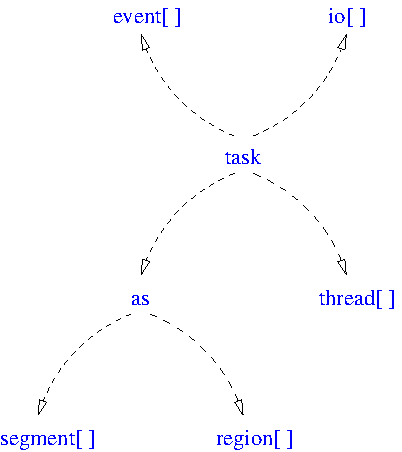
\includegraphics[scale=0.7]{\path/figures/objects-hierarchy.pdf}
    \caption{kaneton objects hierarchy.}
    \label{figure:objects-hierarchy}
  \end{center}
\end{figure}

XXX

overview: kernel = arch + generic :: data-struct + proc
expliquer ca dans overview pour introduire les sets!

XXX

There is another kaneton object which is internally widely used: the
\textbf{set} object. A \textit{set} object is an abstract data structure
managed by a dedicated manager, the \textit{set manager}. The \textit{set
manager} is used by the other kaneton managers for storing data without taking
care of how it is technically done. The set concept was introduced to make the
microkernel code as clear as pseudo code. For more information on the
\textit{set manager}, please refer to the book \textit{The kaneton
microkernel :: core}.

The kaneton microkernel was designed to be ported on many different - existing
or not - architectures. Therefore, the microkernel is divided into two
major components: the \textbf{core} and the \textbf{machine}. The \textit{core}
designs the kaneton source code which is independent from the underlying
computer. For more information on the \textit{core} component, please refer
to the appopriate book \textit{The kaneton microkernel :: core}. On the
contrary, the \textit{machine} component contains the source code related to
the underlying specific hardware.

Since a microprocessor architecture can be used on different mother boards
with various chipsets, the \textit{machine} component is also divided into
a \textbf{platform} which represents the board package; and a
\textbf{architecture} which represents the microprocessor.

Note that the behaviour of the \textit{machine} component can change depending
on the \textit{platform}/\textit{architecture} coupling. Therefore, the
\textbf{glue} was introduced to deal with the multiple
\textit{platform}/\textit{architecture} combinations.

\textit{Figure XXX} illustrates this decomposition. For more information on
the portability system, please refer to the \textit{Chapter
\ref{chapter:portability}}.

XXX [figure]

The kaneton microkernel provides powerful features for distributing computing
including security through capabilities but also communication through a
complete message passing system. Additionally, the microkernel already
integrates the notion of communicating node. As such, the microkernel knows
that the \textbf{distributed system} is composed of
  \textbf{machines}\footnote{The term \textit{machine} is used to represents
                             both the architecture-dependent microkernel's
                             source code and a computer in the distributed
                             system.},
each machine running a kaneton microkernel-based operating system. Moreover,
the communicating \textit{tasks} are named \textbf{nodes} in the distributed
system context.

\textit{Figure XXX} illustrates a distributed system composed of \textit{five}
machines and multiple \textit{nodes} which communicate with each other.

XXX [figure]

The kaneton microkernel is not directly launched when the computer is
turned on. Indeed, a \textbf{bootloader} first set up an execution environment
so that the kernel can be launched properly. The \textit{bootloader} takes
some \textbf{inputs} which represents additional files: configuration
files, execution files etc. For example, the first \textit{input} the
\textit{bootloader} uses is the kaneton microkernel binary file which is
loaded and launched by the \textit{bootloader} itself.

The kaneton microkernel manages tasks which are classified into \textit{four}
categories according to the privileges they get on the system. These different
classes of task are described next.

A \textbf{program} is the lowest priviliged task of the system. The common
user programs are the well known UNIX{\copyright} binaries like
\textit{/bin/ls}, \textit{/bin/sh} etc. A \textbf{service} is a microkernel
server which provides a logical service. For example, a service could be the
\textit{Virtual File System} which dispatches the calls to the file systems
servers. A \textbf{driver} is a service which performs hardware communication.
For example, a \textit{Wireless driver} is a \textit{driver} in the kaneton
terms. Finally, a \textbf{kernel} is a task which is a kind of super-driver
in which it has full rights on the whole underlying hardware.

For more information on the design on the kaneton microkernel, please
refer to the paper \textit{The kaneton microkernel project}.

%
% implementation
%

\section{Implementation}

This section focuses on the terminology used in the \textit{kaneton microkernel
research project} implementation. Obviously, this terminology is also used
in the educational project's context.

As explained in the previous section, the kaneton microkernel is subdivided
into multiples managers.

Each manager provides an interface to manipulate the kaneton object or
something the manager is in charge. The naming scheme used for these provided
functions is detailed below.

Recall that the interface provided by the set of kaneton managers is not
absolutely identical to the system call interface. Indeed, some functions
are private to the microkernel. Moreover, some functions of a manager's
interface must only be called by the manager itself and should not be called
by the other managers.

The couple of functions \textbf{initialize}() and \textbf{clean}() initialize
and clean the manager, respectively.

The function \textbf{show}() displays information on a given identified object
while the function \textbf{dump}() displays information on every objects
hold by the manager.

The function \textbf{reserve}() reserves an object given some properties. On
the contrary, the function \textbf{release}() releases it.

The function \textbf{clone}() clones an object. It is important to understand
that cloning an object does not just mean generating an identical object.
Indeed, cloning an object implies cloning every object this object holds or
depends on.

The function \textbf{give}() gives an object to another entity. The function
\textbf{flush}() cleans every object previously reserved.

The function \textbf{get}() is used to retrieve a kaneton object given its
identifier. Note that this function is private to the manager.

In addition, the kaneton managers generally provide functions for modifying
a property of a given identified object. Moreover, every manager provides
a function \textbf{attribute}() which can be used to retrieve the state
of an object's property.
